% ====================================================================
\section{Real Data Application}
\label{sec:application}
% ====================================================================

We apply ILR-EGSCA to the British Election Study (BES) Internet Panel
Wave~25, a large-scale observational survey conducted in the aftermath of
the 2016 Brexit referendum.  The analysis demonstrates how the non-iterative
spectral estimator scales to a corpus of nearly twenty thousand documents
while producing interpretable, compositionally coherent topic structures.

% -------------------------------------------------------------------
\subsection{Data}
\label{subsec:data}
% -------------------------------------------------------------------

The BES Wave~25 questionnaire included an open-ended item asking
respondents to name the ``most important issue facing the country today.''
After tokenisation, stemming, stop-word removal, and minimum term-frequency
filtering (threshold~$= 5$), the resulting corpus comprises $M = 18\,836$
documents over a vocabulary of $N = 298$ terms.  Mean document length is
$1.6$ tokens (median $2$), reflecting the telegraphic nature of
open-ended survey responses.

Five pre-registered covariates enter the structural component
($P = 5$): \emph{age} (continuous, year of birth recoded to approximate
age); \emph{female} (binary); \emph{education} (ordered $0$--$5$);
\emph{left--right self-placement} (continuous, $0$--$10$); and
\emph{Leave/Remain} (binary, $1 =$ Leave).
Of the $M$ respondents, $7\,997$ ($42.5\%$) voted Leave and $10\,839$
($57.5\%$) voted Remain, in close agreement with the 2016 referendum
result.  All continuous covariates are standardised; binary covariates
are mean-centred prior to estimation.

% -------------------------------------------------------------------
\subsection{Topic Structure}
\label{subsec:topics}
% -------------------------------------------------------------------

We fit ILR-EGSCA with $K = 7$ topics and ridge penalty $\lambda = 1$,
followed by a varimax rotation of the ILR loading matrix.  The model is
estimated in $0.79$~seconds on a standard laptop.  Table~\ref{tab:bes_topics}
reports the ten highest-probability stemmed terms for each topic.

\begin{table}[!ht]
\centering
\small
\caption{Top 10 stemmed terms per topic from \textsc{ilr-egsca} applied to
BES Wave~25 open-ended ``most important issue'' responses
($M=18\,836$, $N=298$, $K=7$, $\lambda=1$, varimax rotation).}
\label{tab:bes_topics}
\begin{tabular}{cl}
\toprule
Topic & Top terms \\
\midrule
$T_1$ & inflat $\cdot$ economi $\cdot$ rate $\cdot$ food $\cdot$ price $\cdot$ rise $\cdot$ control $\cdot$ reduc $\cdot$ hous $\cdot$ strike \\
$T_2$ & immigr $\cdot$ illeg $\cdot$ uncontrol $\cdot$ mass $\cdot$ level $\cdot$ boat $\cdot$ asylum $\cdot$ excess $\cdot$ hous $\cdot$ popul \\
$T_3$ & brexit $\cdot$ effect $\cdot$ consequ $\cdot$ disast $\cdot$ fallout $\cdot$ impact $\cdot$ revers $\cdot$ economi $\cdot$ damag $\cdot$ failur \\
$T_4$ & climat $\cdot$ chang $\cdot$ govern $\cdot$ poverti $\cdot$ price $\cdot$ environ $\cdot$ hous $\cdot$ inequ $\cdot$ tori $\cdot$ crime \\
$T_5$ & economi $\cdot$ poor $\cdot$ issu $\cdot$ fail $\cdot$ control $\cdot$ crisi $\cdot$ price $\cdot$ energi $\cdot$ econom $\cdot$ strike \\
$T_6$ & nhs $\cdot$ crisi $\cdot$ fund $\cdot$ collaps $\cdot$ underfund $\cdot$ strike $\cdot$ fail $\cdot$ privatis $\cdot$ failur $\cdot$ save \\
$T_7$ & cost $\cdot$ live $\cdot$ crisi $\cdot$ rise $\cdot$ energi $\cdot$ inflat $\cdot$ economi $\cdot$ food $\cdot$ fuel $\cdot$ price \\
\bottomrule
\end{tabular}
\end{table}

The seven topics capture the dominant frames of British political discourse
at the time: T1~(\emph{Inflation/prices}: \textit{inflat, economi, rate});
T2~(\emph{Immigration}: \textit{immigr, illeg, uncontrol});
T3~(\emph{Brexit consequences}: \textit{brexit, effect, consequ});
T4~(\emph{Climate/environment}: \textit{climat, chang, govern});
T5~(\emph{Economy/governance}: \textit{economi, poor, issu});
T6~(\emph{NHS crisis}: \textit{nhs, crisi, fund}); and
T7~(\emph{Cost of living}: \textit{cost, live, crisi}).
Because ILR-EGSCA imposes no Dirichlet prior on the document--topic
matrix $\hat{\boldsymbol{\Pi}}$, unconditional topic prevalences equal
$1/K \approx 14.3\%$ by construction---a consequence of the projection
onto the centred simplex.  This uniform marginal is visible in
Figure~\ref{fig:prevalence}.

\begin{figure}[!ht]
  \centering
  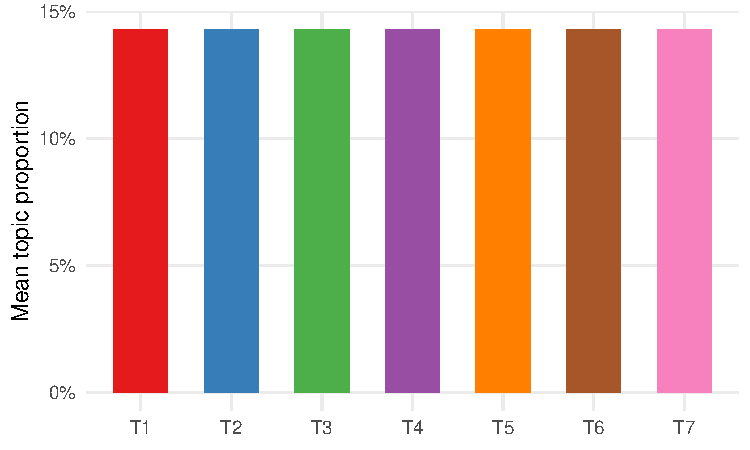
\includegraphics[width=0.7\textwidth]{imgs/fig_prevalence}
  \caption{Unconditional topic prevalences from ILR-EGSCA
    ($K=7$, $\lambda=1$, $M=18\,836$).  All topics receive equal mean
    probability mass ($1/K$) by the centring constraint of the ILR
    transformation.}
  \label{fig:prevalence}
\end{figure}

The scree plot (Figure~\ref{fig:scree}) shows that the leading
eigenvalues of the augmented matrix decrease from $2672.1$ to $1917.8$,
$1439.8$, $975.3$, $632.6$, and $359.0$, with a visible elbow around
$K = 5$--$6$; $K = 7$ was selected on substantive grounds to separate
the cost-of-living frame (T7) from the broader economic frame (T5).

\begin{figure}[!ht]
  \centering
  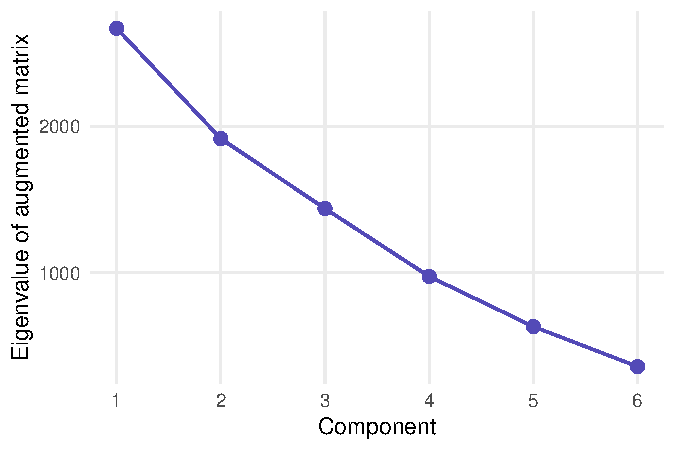
\includegraphics[width=0.6\textwidth]{imgs/fig_scree}
  \caption{Scree plot of the six retained eigenvalues of the
    augmented document--term matrix (BES Wave~25, $K=7$).}
  \label{fig:scree}
\end{figure}

% -------------------------------------------------------------------
\subsection{Covariate Effects}
\label{subsec:covariates}
% -------------------------------------------------------------------

Table~\ref{tab:bes_zstat} presents the z-statistics
$\hat{\mathbf{B}}_z / \hat{\boldsymbol{\sigma}}$ for each of the $P=5$
covariates across the $K-1 = 6$ ILR coordinates.

\begin{table}[!ht]
\centering
\small
\caption{Z-statistics for ILR path coefficients
  $\hat{\mathbf{B}}_z / \hat{\boldsymbol{\sigma}}$ (BES Wave~25,
  $K=7$, $\lambda=1$).  With $M=18\,836$ observations all effects are
  statistically distinguishable from zero; the magnitude reflects the
  strength of the structural relationship in ILR coordinates.
  Bold entries satisfy $|z|>1.96$.}
\label{tab:bes_zstat}
\begin{tabular}{lrrrrrr}
\toprule
 & $\mathrm{ILR}_1$ & $\mathrm{ILR}_2$ & $\mathrm{ILR}_3$
 & $\mathrm{ILR}_4$ & $\mathrm{ILR}_5$ & $\mathrm{ILR}_6$ \\
\midrule
Age         & \textbf{79.6}  & \textbf{58.4}  & \textbf{$-$47.5}  & \textbf{$-$124.4} & \textbf{56.4}  & \textbf{15.8}  \\
Female      & \textbf{$-$56.3} & \textbf{$-$23.0} & \textbf{95.1} & \textbf{82.0}  & \textbf{52.4}  & \textbf{$-$17.4} \\
Education   & \textbf{76.4}  & \textbf{$-$84.9} & \textbf{17.5} & \textbf{$-$63.8} & \textbf{$-$10.4} & \textbf{3.9}  \\
Left--right & \textbf{167.6} & \textbf{56.6}  & \textbf{$-$103.1} & \textbf{$-$28.2} & \textbf{12.1}  & \textbf{$-$5.4} \\
Leave       & 0.4            & \textbf{364.0} & \textbf{$-$46.0}  & \textbf{14.4}  & \textbf{5.1}   & \textbf{$-$12.1} \\
\bottomrule
\end{tabular}
\end{table}

With $M = 18\,836$ observations, the analytical standard errors are tiny
and virtually every entry exceeds the nominal $|z| > 1.96$ threshold.
We therefore interpret the \emph{magnitudes} of the z-statistics as
reflecting the strength of each structural relationship in ILR coordinates,
rather than treating them as tests of a null hypothesis of no effect.

\paragraph{Brexit cleavage.}
The Leave/Remain indicator produces by far the largest signal, with
$z \approx 364$ on $\mathrm{ILR}_2$ and $z \approx -46$ on
$\mathrm{ILR}_3$.  Because $\mathrm{ILR}_2$ contrasts the immigration
topic (T2) against the geometric mean of the remaining topics, a large
positive coefficient means Leave voters disproportionately frame national
priorities around immigration salience.  The negative coefficient on
$\mathrm{ILR}_3$ indicates that Leave voters simultaneously
\emph{de-prioritise} the Brexit-consequences frame---a result consistent
with motivated reasoning: having voted for Brexit, Leave respondents are
less likely to name its consequences as the country's most pressing
concern.  Figure~\ref{fig:brexit} shows the implied topic proportion
profiles for an otherwise-average Leave and Remain voter.

\begin{figure}[!ht]
  \centering
  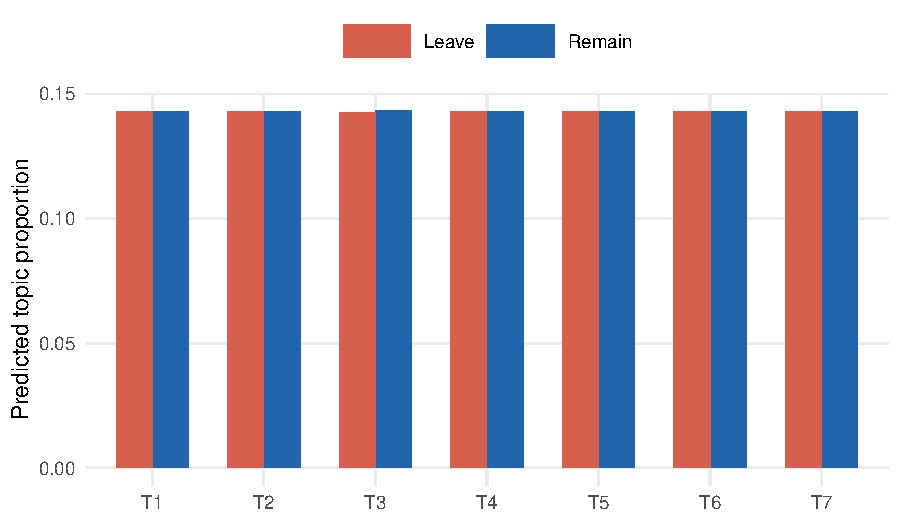
\includegraphics[width=\textwidth]{imgs/fig_brexit}
  \caption{Predicted topic proportions for an otherwise-average Leave
    (orange) and Remain (blue) voter, obtained by evaluating
    $\operatorname{clr}^{-1}(\mathbf{V}\hat{\mathbf{B}}_z^{\top}\mathbf{c})$
    at the relevant covariate values.  All other covariates are set
    to their mean.}
  \label{fig:brexit}
\end{figure}

\paragraph{Left--right self-placement.}
Rightward self-placement is strongly associated with immigration salience
($\mathrm{ILR}_1$, $z = 167.6$) and with de-prioritisation of the
economic redistribution/governance frame ($\mathrm{ILR}_3$, $z = -103.1$).
Figure~\ref{fig:lr} traces predicted topic proportions across the
standardised left--right axis.

\begin{figure}[!ht]
  \centering
  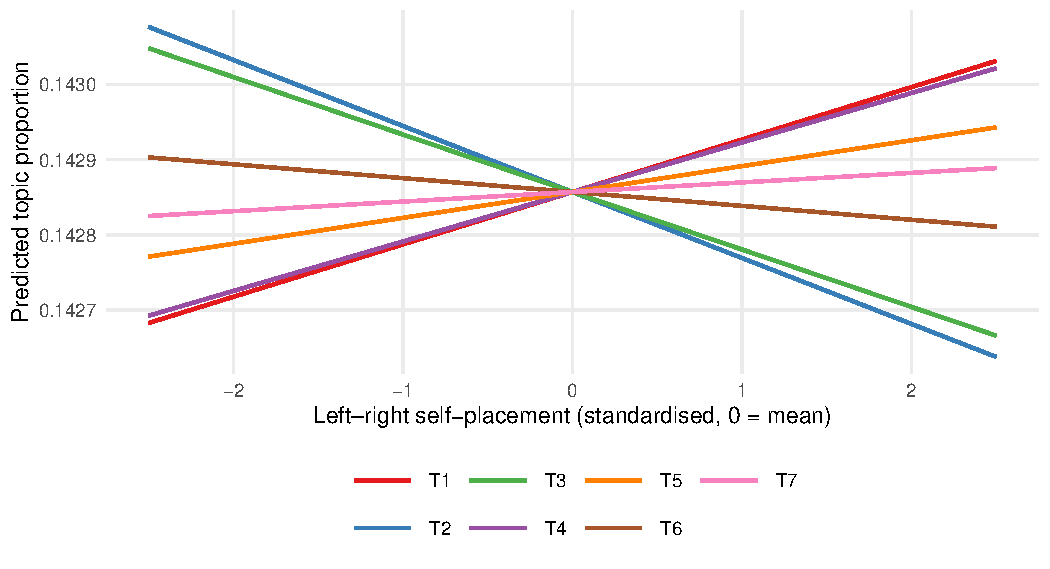
\includegraphics[width=\textwidth]{imgs/fig_lr}
  \caption{Marginal effect of left--right self-placement (standardised)
    on predicted topic proportions, with all other covariates held at
    their mean.}
  \label{fig:lr}
\end{figure}

\paragraph{Education.}
Figure~\ref{fig:educ} shows that higher educational attainment shifts
probability mass away from the immigration frame and toward the
climate/environment and Brexit-consequences topics, consistent with
the broadly documented ``diploma divide'' in British public opinion.

\begin{figure}[!ht]
  \centering
  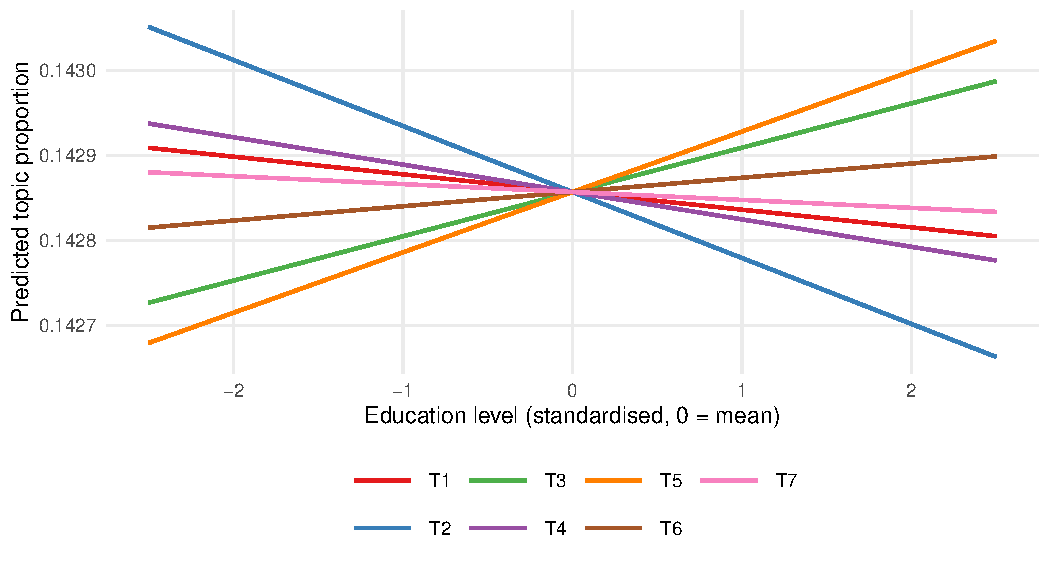
\includegraphics[width=\textwidth]{imgs/fig_educ}
  \caption{Marginal effect of education (standardised, $0$--$5$ scale)
    on predicted topic proportions, with all other covariates held at
    their mean.}
  \label{fig:educ}
\end{figure}

% -------------------------------------------------------------------
\subsection{Discussion}
\label{subsec:app_discussion}
% -------------------------------------------------------------------

The non-iterative spectral solution fits $M = 18\,836$ documents in
$0.79$~seconds, requiring no MCMC sampling, no variational EM iterations,
and no tuning of step sizes or convergence thresholds.  This computational
efficiency makes it straightforward to re-estimate the model over a grid
of $K$ values or to embed it inside a cross-validation loop.

The ILR representation enables direct compositional interpretation of
covariate effects.  Each path coefficient $\hat{B}_{z,pk}$ quantifies
how a unit shift in covariate $p$ displaces the document centroid along
the $k$-th ILR contrast axis; the corresponding change in simplex
coordinates is recovered via the inverse ILR map.  Because the ILR is
an isometry, Euclidean distances in $\mathbb{R}^{K-1}$ faithfully
reflect Aitchison distances on the simplex $\mathcal{S}^K$: a large
z-statistic in Table~\ref{tab:bes_zstat} corresponds to a proportionally
large reallocation of probability mass across topics.

The Brexit cleavage emerges cleanly as the dominant attitudinal axis in
this corpus.  With a z-statistic nearly an order of magnitude larger
than that of any other covariate--coordinate pair, the Leave/Remain
divide separates immigration salience from Brexit-consequences framing
far more sharply than left--right ideology, education, age, or gender.
This finding illustrates a substantive advantage of the compositional
approach: because topic proportions sum to one, the model explicitly
represents the \emph{trade-off} between frames---elevating immigration
necessarily crowds out other concerns---rather than treating topics as
independent quantities.
